\section{Konzept eines innovativen Studiengangsfinders}
\subsection{Vorstellung der OTH-Regensburg als Fallbeispiel}
Die Ostbayerische Technische Hochschule Regensburg (OTH-Regensburg) dient in
dieser Masterarbeit als praxisorientiertes Fallbeispiel für die Konzeption und 
Umsetzung eines innovativen Studiengangsfinders.

\subsubsection{Über die OTH-Regensburg}
Die OTH-Regensburg, gegründet im Jahr 1971, ist eine der größten Hochschulen
für angewandte Wissenschaften in Deutschland. Mit ihrem breiten Spektrum an 
praxisorientierten Studiengängen und ihrer engen Verbindung zur Industrie bietet
die OTH-Regensburg eine ideale Umgebung für die Entwicklung und Implementierung
eines innovativen Studiengangsfinders. \parencite{regensburg_oth_2023}

Die Hochschule zeichnet sich durch eine moderne Infrastruktur, hochqualifizierte 
Dozenten und eine enge Zusammenarbeit mit regionalen Unternehmen aus. Mit mehr
als 50 Bachelor- und Masterstudiengängen in den Bereichen
Ingenieurwissenschaften, Naturwissenschaften, Wirtschaft und
Sozialwissenschaften bietet die OTH-Regensburg eine breite Palette an 
Studienmöglichkeiten. \parencite{regensburg_oth_2023}

\subsubsection{Herausforderung und Zielsetzung}
Wie viele Bildungseinrichtungen steht auch die OTH-Regensburg vor der
Herausforderung, ihre Vielzahl an Studiengängen für Studieninteressierte
transparenter und zugänglicher zu machen. Der Studiengangsfinder, der im Rahmen
dieser Masterarbeit entwickelt wird, soll dazu beitragen, potenziellen
Studierenden eine klarere Orientierung über die verfügbaren Studienmöglichkeiten
zu bieten und ihre Entscheidungsfindung zu unterstützen.

Durch die Anwendung des Studiengangsfinders StudyMap an der OTH-Regensburg wird nicht nur ein innovatives Werkzeug für Studieninteressierte geschaffen, sondern auch die Effektivität und Transparenz der Studienorientierung an der Hochschule selbst verbessert. Die Integration und algorithmische Verarbeitung von Daten zu Studiengängen und Schwerpunkten ermöglicht eine präzisere Darstellung der Studienvielfalt und fördert gleichzeitig die strategische Ausrichtung der Hochschule.

\subsection{Konzept für eine automatisch generierte Infografik}\label{sec:konzept}
Die Grundlage für das Konzept der automatisch generierten Infografik bildet die methodische Vorarbeit, die in den vorhergehenden Kapiteln detailliert erläutert wurde. Im Zuge der Methodik, wie in Kapitel \ref{sec:methodik} beschrieben, wurden Studiengänge anhand verschiedener Kategorien bewertet und mithilfe des MDS-Algorithmus in zweidimensionale Koordinaten transformiert. Das daraus resultierende Zahlenmaterial bildet die Grundlage für die Visualisierung in der Infografik. In den folgenden Unterkapiteln wird ein erstes Designkonzept für die Software vorgestellt.

\subsubsection{Visualisierung der Studiengänge}

\begin{figure}[H]
    \centering
    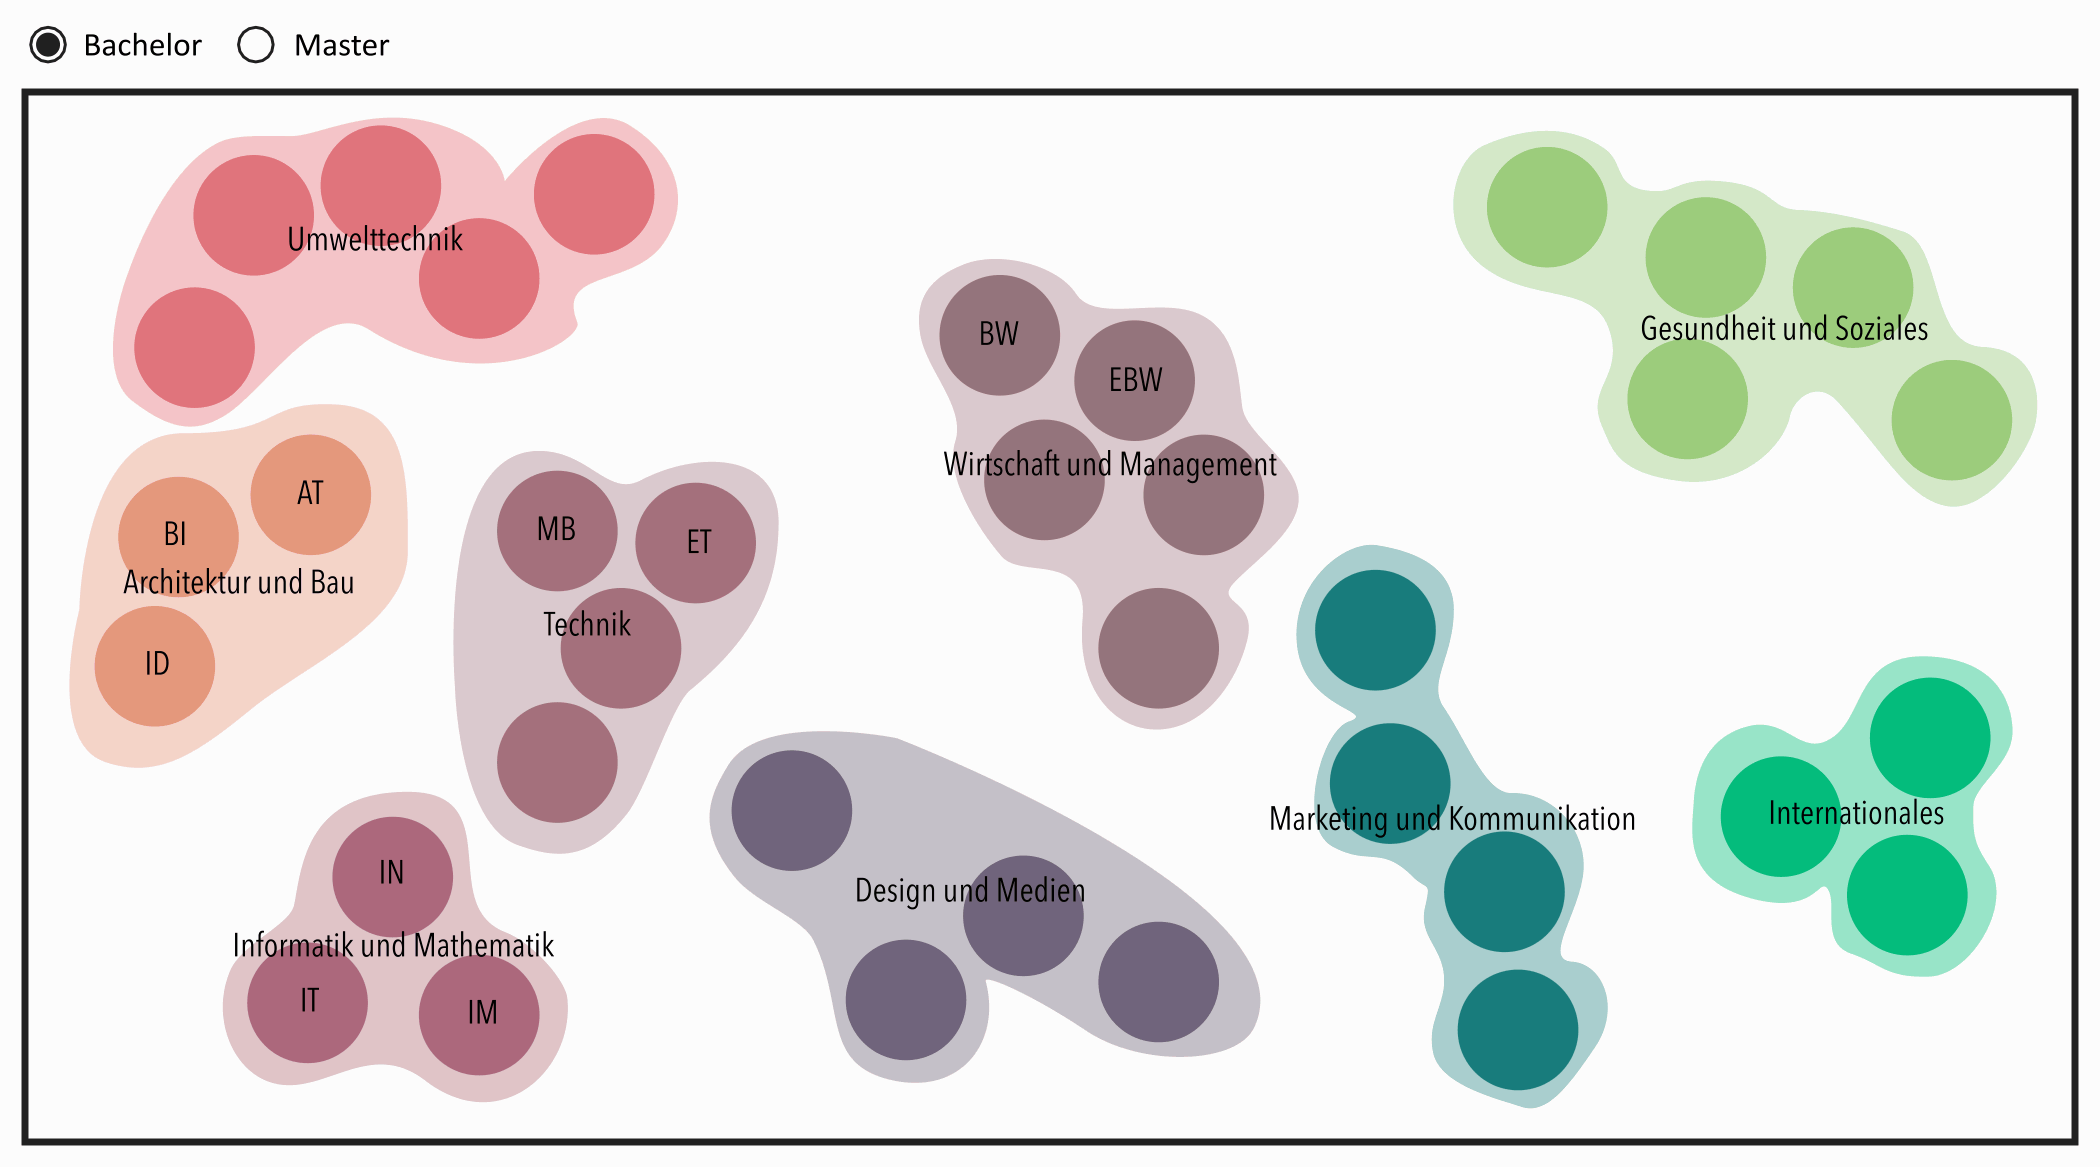
\includegraphics[width=\textwidth]{mockup_bubbles}
    \caption{Erstes Mockup einer möglichen Implementierung}
    \bildquelle{Eigene Darstellung}
    \label{fig:mockup-bubbles}
\end{figure}

\autoref{fig:mockup-bubbles} zeigt das Mockup des Studiengangsfinders StudyMap. Ein Mockup ist eine Darstellung eines Produkts, wie beispielsweise einer App oder Website, die zeigt, wie das finale Produkt aussehen könnte. Mockups sind statische Designkonzepte, die sich von Wireframes, die nur das Grundgerüst darstellen, dadurch unterscheiden, dass sie bereits sehr detailliert ausgearbeitet sind. \parencite{coursera_staff_what_2023}

Das Mockup präsentiert die Vielfalt der Studiengänge auf eine möglichst anschauliche Weise. Dabei werden inhaltlich ähnliche Studiengänge in Form von sogenannten \glqq Bubbles\grqq{} in unmittelbarer Nähe  zueinander positioniert (siehe \autoref{fig:mockup-bubbles}). Die Bubbles enthalten jeweils die Kürzel der Studiengänge. Exemplarisch enthalten in \autoref{fig:mockup-bubbles} nur einige wenige Bubbles ein Kürzel.

\subsubsection{Berücksichtigung von Schwerpunkten}
Ein wesentlicher Aspekt des Infografik-Konzepts ist die Berücksichtigung von 
Schwerpunkten. Die Supergruppen, die in der Datenverarbeitung definiert wurden, 
werden hier als leichter Schleier um die darin beinhalteten Studiengänge 
präsentiert (siehe \autoref{fig:mockup-bubbles}). Außerdem werden alle
Supergruppen mit einer zentrierten Beschriftung versehen. Dies ermöglicht es den
Nutzern, gezielt nach Studiengängen innerhalb bestimmter Kategorien zu suchen
und ihre Präferenzen entsprechend auszurichten.

\subsubsection{Interaktivität}
StudyMap wird durch interaktive Elemente angereichert, um den Nutzern eine individuelle Erkundung der Daten zu ermöglichen. Beispielsweise können durch Mausklicks zusätzliche Informationen zu einem Studiengang abgerufen werden.

\begin{figure}[H]
    \centering
    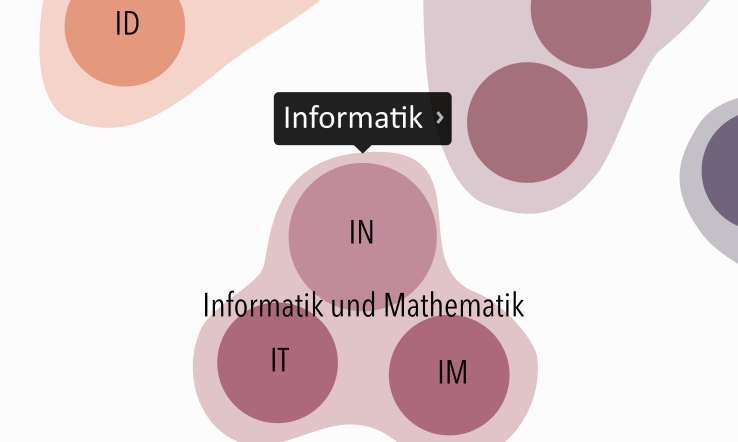
\includegraphics[width=0.5\textwidth]{mockup_bubbles_hover}
    \caption{Mockup: Tooltip über Bubble}
    \bildquelle{Eigene Darstellung}
    \label{fig:mockup-bubbles-hover}
\end{figure}

Sobald ein Benutzer auf einem Desktop-Gerät (z.B. Laptop) mit der Maus über eine
Bubble fährt, erscheint ein Tooltip mit dem vollständigen Namen des Studiengangs
(siehe \autoref{fig:mockup-bubbles-hover}). Ein Tooltip ist ein grafisches
Element, das zusätzliche Informationen zu einem Objekt liefert \parencite{joyce_tooltip_2019}. Aufgrund der fehlenden Maus auf
mobilen Endgeräten, erscheint der Tooltip darauf erst beim Klick auf eine
Bubble. 

Möchte der Studieninteressierte mehr über den Studiengang erfahren, bietet das
Konzept zusätzlich die Möglichkeit, ein Popup mit Details zu öffnen (siehe
\autoref{fig:mockup-bubbles-popup}). Bei Desktop-Geräten genügt ein einfacher
Klick auf die Bubble oder den sich öffnenden Tooltip, bei mobilen
Endgeräten ist ein zweiter Klick auf die jeweiligen Elemente erforderlich.

\begin{figure}[H]
    \centering
    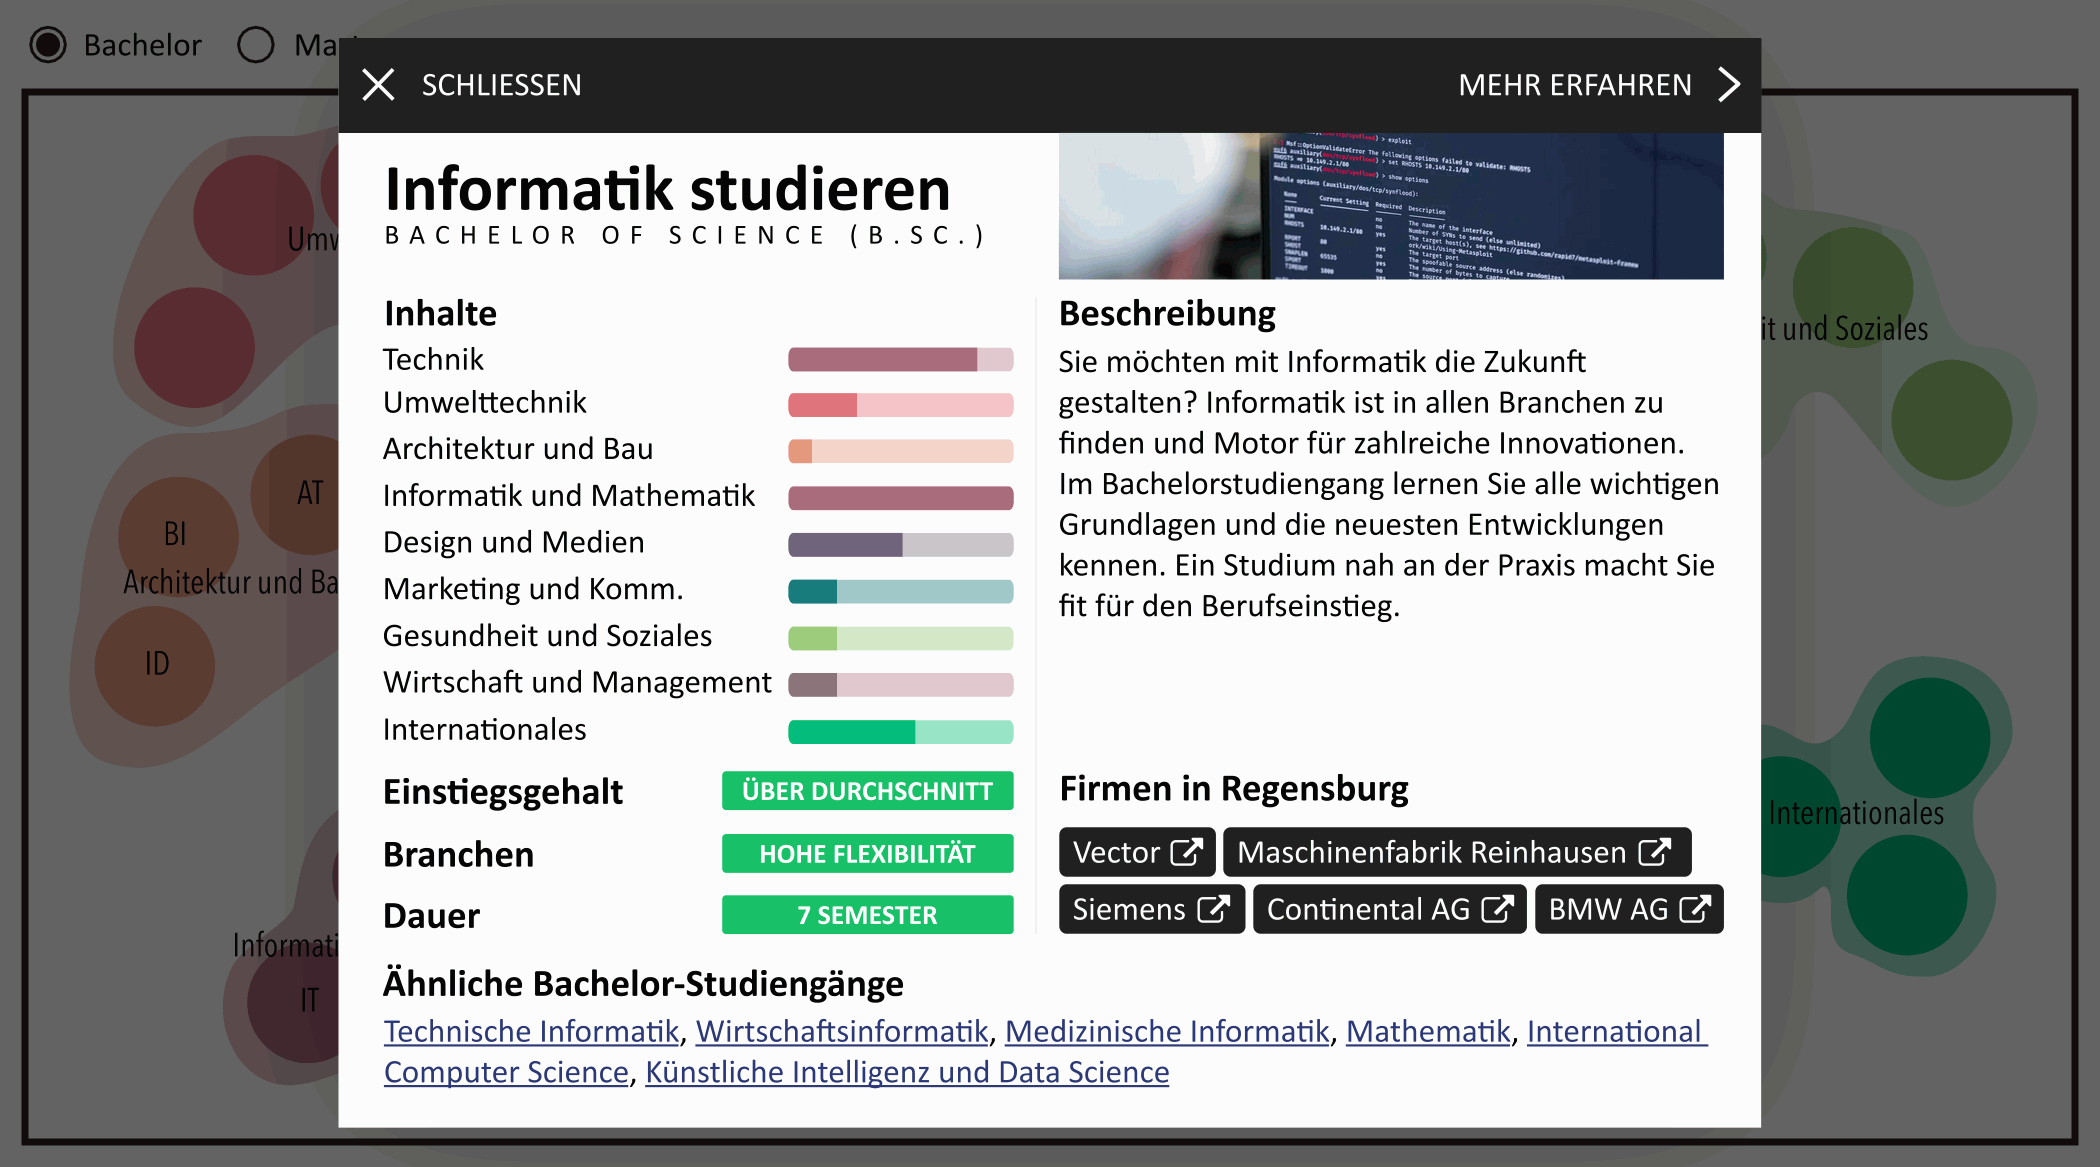
\includegraphics[width=\textwidth]{mockup_bubbles_popup}
    \caption{Mockup: Popup mit Details eines Studiengangs}
    \bildquelle{Eigene Darstellung}
    \label{fig:mockup-bubbles-popup}
\end{figure}

Im Folgenden wird das Konzept des Popup-Dialogs beschrieben, welches in \autoref{fig:mockup-bubbles-popup} visualisiert ist.

Innerhalb des Popups findet der Nutzer eine prägnante Kurzbeschreibung des Studiengangs. Die Inhaltskategorien werden durch Fortschrittsbalken visualisiert, die den Anteil der verschiedenen Kategorien anzeigen. So kann beispielsweise die Kategorie \glqq Informatik\grqq{} zu 90\% ausgefüllt sein, um den Schwerpunkt des Studiengangs zu verdeutlichen.

Zusätzlich liefert das Popup Informationen über Einstiegsgehälter, relevante Branchen, Studiendauer und ähnliche Studiengänge. Letztere werden nicht statisch dargestellt, sondern vom Algorithmus dynamisch berechnet, um stets aktuelle und präzise Informationen zu liefern.

Darüber hinaus wird eine Liste von Unternehmen in Regensburg angezeigt, die gezielt nach Absolventen dieses Studiengangs suchen. Dieser Aspekt gibt dem Nutzer einen Einblick in potentielle Arbeitgeber und eröffnet berufliche Perspektiven direkt in der Region.

Durch die Integration dieses Fensters wird die Benutzerfreundlichkeit erheblich 
verbessert, da der Nutzer einen tieferen Einblick in die einzelnen Studiengänge
erhält, ohne die Seite wechseln zu müssen.

\subsection{Datenpflege und -sicherung}
Um StudyMap stets mit aktuellen Daten betreiben zu können, müssen diese gepflegt werden. Wie in \autoref{sec:herkunft-der-daten} erläutert, stammen die Daten bisher von der Vizepräsidentin der OTH-Regensburg. Zum Datum der Arbeit ist die Person oder Personengruppe, die in Zukunft für das Projekt verantwortlich sein wird, noch nicht bekannt.

\subsubsection{Verwaltungssoftware vs. Anleitung}\label{sec:verwaltungssoftware}
Aufgrund des technischen Aufwands beim Einpflegen der Daten per SSH- und SCP-Verbindung sowie dem manuellen Aufruf des Python-Skripts zur Generierung der Positionsdaten wird hier eine Unterstützung benötigt. Während SSH (Secure Shell) dazu da ist eine verschlüsselte Verbindung zur Kommandozeile des Servers aufzubauen, ermöglicht SCP (Secure Copy) den sicheren Austausch von Dateien mit dem Server.

Bei einer manuellen Aktualisierung der Daten über SCP müssen die neuen Dateien per Kommandozeile auf den Server kopiert werden. Anschließend ist das Python-Skript mit den richtigen Parametern aufzurufen, um den Prozess zu starten. Um die im nächsten Abschnitt beschriebene Produktiv- und Staging-Umgebung einzuhalten, sind außerdem verschiedene Ordnerstrukturen zu beachten.

Der technische Hintergrund der Person, die das Projekt in Zukunft betreuen wird, ist ungewiss. Daher sollte ein Verwaltungstool zur Vereinfachung des Pflegeprozesses entwickelt werden. Die Alternative einer Anleitung in Form eines PDF-Dokuments könnte aufgrund der Komplexität der Vorgänge schnell zu kompliziert und umständlich werden. Des Weiteren erhöht sich bei jedem manuell zu erledigenden Schritt die Wahrscheinlichkeit für Fehler.

\subsubsection{Staging- und Produktivumgebung}
In diesem Abschnitt wird der Bedarf einer Trennung zwischen Staging- und Produktivumgebung erläutert. Unter einer Staging-Umgebung versteht man in der Informatik ein Testsystem, welches unter annähernd realen Bedingungen erlaubt die Anwendung zu testen - meist ist diese nur über einen speziellen Zugang für authentifizierte Personen erreichbar. Die Produktivumgebung hingegen bezeichnet die für die Öffentlichkeit freigegebene Version der Software.

Aufgrund der Komplexität des Algorithmus ist der Prozess der Positionsberechnung für einen Menschen nicht deterministisch nachvollziehbar. Daher ist eine Testumgebung erforderlich. Im ungünstigsten Fall überlappen sich die Bubbles im Canvas bei vorheriger ähnlicher Bewertung der Studiengänge. Für diesen Fall muss eine Staging-Umgebung zur Verfügung stehen, auf der ein neuer Datensatz getestet werden kann. Sobald dieser optimiert und von den verantwortlichen Personen freigegeben wird, sollte der Staging-Datensatz per Knopfdruck in die Produktivumgebung überführt werden können.

Dieser zweistufige Prozess erhöht die Fehlersicherheit und ermöglicht es, neue Berechnungen zu testen, ohne sie direkt der Öffentlichkeit zur Verfügung zu stellen.

\subsubsection{Datensicherung}
Neben der im vorigen Abschnitt erläuterten Trennung von Staging- und Produktivumgebung ist ein weiterer wesentlicher Bestandteil des Konzepts die Datensicherung. Sollte trotz Staging-Umgebung ein Fehler auftreten, müssen die alten Daten wiederhergestellt werden können.

Für diesen Fall sieht das Konzept vor, dass bei jeder Produktivschaltung ein Backup der Staging-Version erstellt wird. Dieses Backup sollte im Verwaltungstool per Schaltfläche in die Staging-Umgebung wiederhergestellt werden können. Von dort aus kann es begutachtet und schließlich wieder produktiv geschaltet werden.

Durch diese doppelte Sicherung sollte ein Großteil der versehentlich eingelesenen ungültigen Daten vermieden werden. Zusätzlich muss es immer möglich sein, den aktuell verwendeten Datensatz herunterzuladen. Wenn eine neu zuständige Person den aktuellen Datensatz bearbeiten möchte, kann sie so die aktuell verwendeten Eingabedateien herunterladen und bearbeiten, ohne die vorher dafür zuständige Person kontaktieren zu müssen. Darüber hinaus steht immer ein sogenannter Template-Datensatz zum Download zur Verfügung, der im Falle einer korrupten Datensicherung und einer kaputten Staging- oder Produktivversion einen validen Datenstand als Basis liefert.